\chapter{Command \& Data Handling}%Worked on by Chris+Steph
\setlength{\parindent}{15pt}
\label{ch:avio_grou_hand}


%WE ARE SPECIAL WE DONT NEED THIS :D 
%PLEASE ADHERE TO THIS STRUCTURE
%\section{Design Approach}
  % Talk about literature study etc
%\section{Assumption}
  % We dont have it? 
%\section{Analysis}
  % We dont have it?
%\section{Results}
 %What we have now 
 
\section{Design Approach}

\begin{figure}[htb]
    \centering
    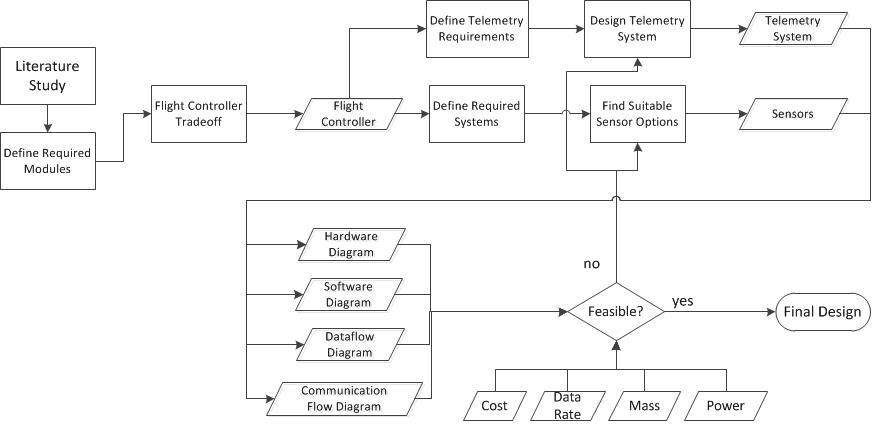
\includegraphics[width=\textwidth]{./CommandDataHandling/Figures/WorkFlow}
    \caption{Command and Data Handling workflow diagram}
    \label{fig:comm_data_work}
\end{figure}



\section{Avionics and Ground Station}%Written by Steph, Chris + Steph responsible/worked on
\label{sec:avio_grou_stat}
In this section, all avionics used in the preliminary design will be explained, as well as the ground handling including payload. In the current phase, several systems were selected. In order to cut down on cost, in future design stages some of the selected systems will be replaced by in-house designed systems. 

An overview of the systems that were selected can be found in \autoref{tab:avio_subs}. This was done based on the requirements %(maybe refer to requirements)
and on extensive online research. Further specifications on the selected systems can also be found here. In \autoref{sec:avio_trad_off} a comparison is made between different available systems. The design of the telemetry system is discussed in \autoref{sec:tele_syst} and in \autoref{sec:grou_stat_layo} the layout of the ground station is explained. Then in \autoref{sec:encr} a secure communication protocol is established. 
\nomenclature[A]{GPS}{Global Positioning System}
\nomenclature[A]{BVLOS}{Beyond Visual Line of Sight}





\begin{table}[h]
    \centering
    \caption{List of avionics subsystem components}
    \label{tab:avio_subs}
    \begin{tabularx}{\textwidth}{>{\small}p{.15\textwidth} >{\small}p{.18\textwidth} >{\small}p{.12\textwidth} L}
    \toprule 
    \textbf{System type}     & \textbf{Selected system} & \textbf{Price} &\textbf{System specifications} 
    \\ \midrule
    Flight control module      & Pixhawk 2.1\footnotemark & USD 198,- & Isolated IMU (3x accelerometer, 3x gyroscope, 3x magnetometer, 2x barometer), flight controller board, multiple input ports, micro SD card for internal memory. Estimated size 10x5x2 cm, estimated weight 200 g. %this one goes last when all the others have been filled in
    \\ \hdashline
    Ground avoidance system & SF30-C Laser Rangefinder\footnotemark & USD 699,- & Range 100 m, accuracy $\pm$0.1 m, weight 35 g, dimensions 30 x 55 x 50 mm
    \\ \hdashline 
    Object avoidance system & Jenoptik DLEM 20\footnotemark & Estimated at EUR 1000,- & Sensor uses flight control module for avoidance of obstacles. Dimensions 50 mm x 22 mm x 34 mm, weight 33 g, range 5 km, accuracy 0.5 m.
    \\ \hdashline
    GPS & Here+ GNSS for Pixhawk & USD 48,- & Concurrent reception of up to three GNSS, -167 dBm navigation sensitivity, weight 49 g, dimensions 8x8x2 cm.
    \\ \hdashline
    Radio Control & Frsky V8FR-II receiver\footnotemark & EUR 14,- & 2.4 GHz, Weight 39g, dimensions 34x19x8 mm. 
    \\ \hdashline
    Telemetry & u-Blox TOBY L2-series \footnotemark &   EUR 60,- & Weight 4.8g, dimensions 25x36x3 mm.
    \\ \hdashline
    Payload link & USB or other cable & Estimated at EUR 10,- & Pixhawk module has multiple extra ports for both power and camera modules.
    \\ \midrule
     & Estimated total: & EUR 2000,- & Estimated total size: 400 cm$^3$.
    \\ \bottomrule
    \end{tabularx}
\end{table}


\addtocounter{footnote}{-5}
\stepcounter{footnote}\footnotetext{\url{http://www.robotshop.com/en/pixhawk-21-standard-set.html}, Accessed 12-06-2017}
\stepcounter{footnote}\footnotetext{\url{http://www.robotshop.com/en/sf30-c-laser-rangefinder-100m.html}, Accessed 13-06-2017}
\stepcounter{footnote}\footnotetext{\url{https://www.jenoptik.com/products/defense-and-security/laser-rangefinders/oem-modules-system-integration/dlem}, Accessed 13-06-2017}
\stepcounter{footnote}\footnotetext{\url{https://hobbyking.com/en_us/frsky-v8fr-ii-2-4ghz-8ch-receiver-hv.html}, Accessed 20-06-2017}
\stepcounter{footnote}\footnotetext{\url{https://www.u-blox.com/en/product/toby-l2-series}, Accessed 19-06-2017}

\begin{comment}
http://www.robotshop.com/en/uav-drone-sensors.html
http://pixhawk.org
http://www.robotshop.com/blog/en/how-to-make-a-drone-uav-lesson-4-flight-controller-15191
\end{comment}


\subsection{Trade-off}
\label{sec:avio_trad_off}
In this section, different options for the determination of the avionics systems are discussed. The systems need to be able to measure accelerations, both axial and angular, orientation, altitude, distance to the ground, distance to obstacles and determine its global position. The communication system will be discussed in \autoref{sec:tele_syst}.



In \autoref{tab:flig_cont}, an overview of (combinations of) systems is given that can determine the accelerations, orientation, location and attitude, as well as process all data. This will be the flight control system. For some of the systems the exact size or weight is not known. In these cases, they are not given. Sizes are estimated based on reviews an images. FOOTNOTE


\begin{table}[h]
    \centering
    \caption{Overview of flight control systems}
    \label{tab:flig_cont}
    \begin{tabularx}{\textwidth}{p{.12\linewidth} L  p{.13\textwidth}  }
    \toprule
\textbf{System(s) }     & \textbf{Specifications }       &\textbf{Price, Size}                                %& \textbf{Positives, Negatives}                                                                                        
\\ \midrule
Navio2 Autopilot, Raspberry Pi 3                       & GNSS receiver, extension ports, includes power module, dual IMU, 10 cm resolution barometer, 14 PWM servo outputs, 1.2GHz 64-bit quad-core ARM Cortex-A53 CPU, Integrated 802.11n wireless LAN and Bluetooth 4.1, software still required!                                                                                                                                                                                                                                                                                  & USD253,   2x   55x65x15 mm, 68g                                  % & Provides all desired ports for extra equipment, processor is strong enough. Software still needs to be designed.                                                             
\\ \hdashline             
Radiolink PixHawk 1             & 32bit STM32F427 Cortex M4 corewith FPU, 256KB RAM, 3-axis IMU, 16 bit gyroscope, 14 bit accelerometer and magnetometer                             & USD140                                     %& GPS already included, relatively cheap. Possibly requires extra ports. Also IMUs processing capacity could be better. Software available 
\\ \hdashline
Lynxmotion Quadrino     & Nano Drone/UAV Flight Controller, Software included, IMU, Explansion ports, ATmega 2560 (256Kb flash @ 16MHz) Processor.                                                                 & USD150, 53x53x17 mm                                                                                                                           %& Software included.  Meant for smaller category drones, processor might not be able to handle it.    GPS included                                                                  
\\ \hdashline 
MWC MultiWii  & 2 Servo output for camera (only available when using 4 motors or less), Separate 3.3V and 5V LDO voltage regulators                                                                                                                                                                                                                                                  & USD23,      36x36x2 mm                                                                                                               %& Small, cheap.  Output/input port and processing capacity too small, arduino required..                                                                                              
\\ \hdashline
AfroFlight Naze32 Rev6                   & Up to 8 ch RC input, 32-bit processor running at 3.3V/72MHz. BMP280 barometer                                                                                                 & USD21,      36x36 mm,                                                                             7.3g  %& Small, cheap. Meant for quadcopter racing -- not suitable for a lot of data processing.                                                             
\\ \hdashline
DJI Naza-M V2                        & Software included,  Intelligent Orientation Control, PPM, S-BUS \& Ordinary Receiver Supported, Built-in Gimbal Stabilisation Function, Remote Gain Adjustment, Hovering Accuracy (GPS Mode) Vertical:$\pm$0.8m, Horizontal:$\pm$2.5m                                                & USD 159,   4x  45x45x10 mm, 95 g             
                %& Software available, function extensions possible, GPS included. Not very accurate, not certain if CPU can handle all camera data. Relatively large.                              
\\ \hdashline 
Pixhawk 2.1, Here+ GNSS                    & Modular design for flexibility, Triple Redundant IMU system, Modular cube. All inputs/outputs in one single DF17 connector, Concurrent reception of up to three GNSS, -167 dBm navigation sensitivity                                                                                                                                        & USD246, GPS 79x82x17 mm, 49g                                  % & Has a lot of modular options which is ideal for the different payload modules. Also has good processing memory and availability to put in an external memory card.  Relatively large, however would still fit in the design.                                                  
\\ \bottomrule
    \end{tabularx}
\end{table}

\begin{table}[h]
    \setlength\extrarowheight{5pt}
    \setlength\arrayrulewidth{1pt}
    \centering
    \caption{Final Trade-Off}
    \label{tab:avio_trad_off}
    \begin{tabular}{r|
    |>{\centering}p{1cm}
    |>{\centering}p{.5cm}
    |>{\centering}p{2cm}
    |>{\centering}p{1cm}
    |>{\centering}p{.5cm}
    |>{\centering}p{1cm}
    |>{\centering}p{.5cm}
    | c } 
    \raggedright \textbf{Concept \rotatebox{90}{\hspace{0.5cm}Criterion}}        & 
    \rotatebox{90}{\textbf{Size}}                            &
    \rotatebox{90}{\textbf{Cost}}                                   & 
    \rotatebox{90}{\textbf{CPU}}                            & 
    \rotatebox{90}{\textbf{Modularity}}                        & 
    \rotatebox{90}{\textbf{GPS}}                       &
    \rotatebox{90}{\textbf{Accuracy}}                         &
    \rotatebox{90}{\textbf{Software}}       &
    \rotatebox{90}{\textbf{Result}}
    \\\hline
    Navio2      &
    \cellcolor[HTML]{FFC000}-    &
    \cellcolor[HTML]{FFC000}-    &
    \cellcolor[HTML]{00B050}++   &
    \cellcolor[HTML]{00B050}++   &
    \cellcolor[HTML]{92D050}+    &
    \cellcolor[HTML]{92D050}+    &
    \cellcolor[HTML]{FFC000}-    &
    \cellcolor[HTML]{FFFF00}\textbf{55}
    \\[5pt]\hline
    Pixhawk 1          &
    \cellcolor[HTML]{FFFF00}0    &
    \cellcolor[HTML]{FFFF00}0    &
    \cellcolor[HTML]{92D050}+    &
    \cellcolor[HTML]{00B050}++   &
    \cellcolor[HTML]{92D050}+    &
    \cellcolor[HTML]{92D050}+    &
    \cellcolor[HTML]{92D050}+    &
    \cellcolor[HTML]{FFC000}\textbf{33}
    \\[5pt]\hline
    Lynxmotion      &
    \cellcolor[HTML]{92D050}+    &
    \cellcolor[HTML]{FFFF00}0    &
    \cellcolor[HTML]{FFFF00}0    &
    \cellcolor[HTML]{92D050}+    &
    \cellcolor[HTML]{92D050}+    &
    \cellcolor[HTML]{00B050}++   &
    \cellcolor[HTML]{92D050}+    &
    \cellcolor[HTML]{92D050}\textbf{58}
    \\[5pt]\hline
    MultiWii       &
    \cellcolor[HTML]{00B050}++   &
    \cellcolor[HTML]{00B050}++   &
    \cellcolor[HTML]{FF0000}- -   &
    \cellcolor[HTML]{FF0000}- -   &
    \cellcolor[HTML]{FFC000}-    &
    \cellcolor[HTML]{FFFF00}0    &
    \cellcolor[HTML]{00B050}++   &
    \cellcolor[HTML]{FFC000}\textbf{42}
    \\[5pt]\hline
    Afroflight   &
    \cellcolor[HTML]{00B050}++   &
    \cellcolor[HTML]{00B050}++   &
    \cellcolor[HTML]{FF0000}- -   &
    \cellcolor[HTML]{FFC000}-    &
    \cellcolor[HTML]{FFC000}-    &
    \cellcolor[HTML]{FFFF00}0    &
    \cellcolor[HTML]{FFC000}-    &
    \cellcolor[HTML]{00B050}\textbf{81} 
    \\[5pt]\hline
    DJI Naza M   &
    \cellcolor[HTML]{FF0000}- -   &
    \cellcolor[HTML]{FFFF00}0    &
    \cellcolor[HTML]{92D050}+    &
    \cellcolor[HTML]{92D050}+    &
    \cellcolor[HTML]{00B050}++   &
    \cellcolor[HTML]{FF0000}- -   &
    \cellcolor[HTML]{92D050}+    &
    \cellcolor[HTML]{00B050}\textbf{81} 
    \\[5pt]\hline
    Pixhawk 2.1   &
    \cellcolor[HTML]{FFFF00}0    &
    \cellcolor[HTML]{FFC000}-    &
    \cellcolor[HTML]{00B050}++   &
    \cellcolor[HTML]{00B050}++   &
    \cellcolor[HTML]{00B050}++   &
    \cellcolor[HTML]{92D050}+    &
    \cellcolor[HTML]{92D050}+    &
    \cellcolor[HTML]{00B050}\textbf{81} 
    \\[5pt] \hline\hline
    Weight          &
    10              &
    5              &
    20              &
    10              &
    5              &
    10              &
    5           &
    \\[5pt]
    \end{tabular}
\end{table}


It was decided to use a ready-to-use flight control system, instead of installing the different components separately. Therefore, the system needs to consist at least  of an inertia measurement unit (IMU) or accelerometer plus gyroscope to determine accelerations, a compass or magnetometer to determine orientation, a pressure meter and a system that measures the distance to the ground, and preferably a Global Positioning System (GPS). In order to decrease the chance of burnout, a power brick is included in the Pixhawk module to transform the battery voltage to the flight controller voltage and to monitor the battery properties. For object avoidance, two laser sensors will be installed. One with a short range for ground detection, and one able to scan objects that are very far away, for collision avoidance.



\subsection{Telemetry System}%Made by Chris
\label{sec:tele_syst}

In this section, the Radio Control, (RC), system used for Visual Line of Sight, (VLOS), is discussed. Then, different possible telemetry systems for BVLOS communication are introduced and a final system is chosen.

\nomenclature[A]{VLOS}{Visual Line of Sight}

\subsubsection{VLOS}

In order to control the drone in VLOS, a RC receiver is added to the telemetry system of the drone. The main purpose of this receiver is to obtain flight commands send by the operator while in VLOS. 

Although the long range telemetry system in the next section could also be used for this purpose, a RC sender is preferred in close range due to the lower latency (as a direct link is established between operator and drone). Also the reliability of an RC link is higher, as the codes are not modulated and package loss is decreased due to the closer range.     

One disadvantage of the RC link is the fact that it is only used as a one-way link. Measurements of the different sensors are not send towards the ground station and hence it is only used for VLOS control. Data gathered on-board the UAV is send using the cellular link or has to be stored on the internal memory in case the cellular link breaks or is not available.

The most common RC link uses a 2.4 GHz frequency. Comparing different 2.4 GHz receivers, it was concluded, that a Frsky V8FR-II receiver will be used\footnote{\url{https://hobbyking.com/en_us/frsky-v8fr-ii-2-4ghz-8ch-receiver-hv.html}, Accessed 19-06-2017}. It uses eight channels, four used to simultaneously control rudder (change in yaw angle), elevator (change in pitch angle), throttle (change in thrust) and ailerons (change in roll angle). One remaining channel is then used for the tilting mechanisms of the engines, making it possible to manually transition from vertical to horizontal flight. The last three channels can be used for different payload modules which might require some kind of control, this can included opening and closing of the payload bay, rotating of cameras or dropping of payload.


%https://hobbyking.com/en_us/frsky-2-4ghz-accst-taranis-x9d-plus-digital-telemetry-radio-system-mode-2.html


\subsubsection{BVLOS}

The main requirement set for the BVLOS telemetry system is given by requirement SYS-PF-1.3, stating that the UAV, shall be capable of achieving a range of 200 km. As radio frequency communication can not reach these ranges, 2 alternatives are presented in this section: 
\nomenclature[A]{RC}{Radio Control}




\begin{enumerate}
\item{\textbf{Satellite Modem}}

In order to increase the range, a satellite modem could be used. This first sends the data towards a satellite which in turn redirects it towards the drone. The main advantage is that most areas of the Earth are covered and BVLOS operation is thus possible. Using a satellite modem, there are no range limitation. Major disadvantage is the  higher latency, as propagation and processing delays can be up to one second for a geostationary satellite connection. Furthermore, costs for using a satellite link are expensive and data rate dependant. Comparing only the dataflow of the sensors, a constant flow of up to 55 kbps can be necessary (see \autoref{sec:data_hand_bloc_diag}). Using the Iridium satellite network, this results in a cost of around 6 euro per second transmitting all the relevant data, which does not include yet live video feeds or other data consuming devices mounted in the payload.\footnote{\url{http://www.rock7mobile.com/products-rockblock}, Accessed 19-6-2017}

\item{\textbf{GSM/LTE Modem}}

Global System for Mobile Communications, (GSM), and Long Term Evolution, (LTE), modems make use of mobile cellular networks for the data transfer. As mobile telecommunications are widely available nowadays, using a GSM/LTE modem greatly increases the range compared to a radio modem. On top of that, data rates of up to 50 Mbps can be achieved in good conditions.\footnote{\url{https://www.u-blox.com/sites/default/files/TOBY-L2_DataSheet_\%28UBX-13004573\%29.pdf}, Accessed 12-6-2017} Although this makes it possible to use BVLOS operation, cellular networks are less developed in poorer countries and do not cover the oceans at all. This reduces the possible operational area significantly compared to satellite networks. The cost of data services is relatively low compared to satellite links. Several distributors in the Netherlands provide 10 GB of data transfer for around EUR 30,- per month.\footnote{\url{https://www.kpn.com/mobiel/mobiel-internet/simkaart/mobiel-internet-standaard/1-jaar}, Accessed 19-6-2017} 
\end{enumerate}
\nomenclature[A]{GSM}{Global System for Mobile Communications}
\nomenclature[A]{LTE}{Long Term Evolution}
Although the higher coverage of satellite communication is preferred for save and rescue missions, the cost is limited and high data transfer is required in order to obtain a reliable video feed. Furthermore, satellite communications require bigger antennas in order to achieve a safe and reliable data connection. This will increase the final mass, which is not preferred due to requirement SYS-PH-2, which states that the take-off weight should not exceed 25kg. Another major advantage of using cellular networks is the fact that the packages are send using conventional networking technologies and hence also routed this way. This makes it easier to securely deliver the messages, which is in more detail explained in Section \ref{sec:encr}. For these reasons, a GSM/LTE modem is used as larger range telemetry system. This then also comes with the advantage that in order to control and monitor the drone only an internet connection is necessary.

The chosen GSM/LTE modem is a u-Blox TOBY L2-series LTE Modem. It can be connected directly to the Pixhawk Flight Controller via UART. Care should be taken that the correct module is chosen depending on the geographical location where the drone is operating. 

\subsubsection{Final Layout}

Finally, the UAV uses a cellular network connection as main telemetry system. Via an internet connected device, waypoints can be send to the telemetry module for navigation. The flight controller then chooses the best control inputs to perform the mission. Furthermore, higher data rates are supported using this connection, hence also attitude data and monitoring data is send on this channel.

A second, more reliable link is created using the RC connection. This connection can only be used for lower ranges (up to 2 km) and hence it is only used for VLOS. Using the RC channel, the operator can control the thrust as well as pitch, yaw and roll angles. RC communication is thus preferred in case a higher precision is required, as position determination is dependant on GPS accuracy. 

In case the flight controller receives messages from both links, the newest messages are preferred and performed. Furthermore, in case the main cellular link breaks, the flight controller tries to establish a connection with the RC transmitter. If that link is also not available, a return to take-off procedure is performed during which the UAV aborts its mission and returns to its starting point. 


\subsection{Ground Station Layout}%made by Steph
\label{sec:grou_stat_layo}


In this section, the different options for the ground station are discussed, after which a layout for the system is chosen. %maybe mention requirements
The two categories to choose between are a large ground station with a case, displays and controls, or just software that can be installed on any tablet or laptop with an internet connection. It was decided that using software is preferred, since it allows for more flexibility in interfaces and a tablet is easier to transport. Furthermore, as cellular technology is used for communication, only an internet connection is required for control. The only disadvantage is that the UAV will have to rely more on the autopilot, because the inputs given on a tablet will not be control inputs, but waypoints. After some research on world network coverage, it was decided that using just software and a tablet is a viable option\footnotemark.
\footnotetext{\url{http://data.worldbank.org/indicator/IT.CEL.SETS.P2?view=map}, Accessed 12-06-2017}
It was decided to choose a system that is compatible with the Pixhawk system that was selected in \autoref{sec:avio_grou_stat}. Therefore, QGroundControl software will be used\footnotemark. As it is compatible with the Pixhawk, all sensors and equipment connected to it can be incorporated in the program.

\footnotetext{\url{https://docs.qgroundcontrol.com/en/}, Accessed 12-06-2017}

Then, in order to use the more reliable RC Link, as explained in \autoref{sec:tele_syst}, an RC transmitter is needed. A FrSky ACCST TARANIS X9D PLUS Digital Telemetry Radio System\footnotemark is used for this. It supports at least the 8 channels available by the RC receiver and can hence be used for control of the aircraft.

\footnotetext{\url{https://hobbyking.com/en_us/frsky-2-4ghz-accst-taranis-x9d-plus-digital-telemetry-radio-system-mode-2.html}, Accessed 19-06-2017}




\subsection{Encryption}%Made by Chris
\label{sec:encr}

The UAV market is increasing significantly without a major consideration in the safety of the exchanged messages. This comes with the problem that an adversary can without major troubles control the drone. 

A secure communication should be confidential (only the receiver can read the message), authenticated (the receiver is sure who sent the message) and integer (nobody can change the message). However for the flight control communications of the drone it is of no relevance whether an adversary knows that the drone is going to perform a certain action, this section only focuses on authentication and integrity. In case data has to be confidential, it is recommended to look into different encryption techniques using less processing power. 

The protocol used for flight control message exchange is the Micro Air Vehicle Communication, (MAVLink), protocol. It is used for internal communication between the different sensors and the flight controller as well as to transmit useful information as attitude, speed and battery status of the vehicle and to send new waypoints for control of the drone. Although the integrity of the messages is already ensured by the checksum, it only has a length of 2 bytes (16 bits). This checksum can be guessed easily by current computers and hence the scheme is not secure.
\nomenclature[A]{MAVLink}{Micro Air Vehicle Communication}
Integrity and authentication are obtained using a Message Authentication Code (MAC). Before the MAVLink data is send to the cellular network, a Hash-based message authentication code, (HMAC), is attached to it. In order to prevent replay attacks, the current time and date will also be added to the message before calculating the MAC. The HMAC uses the same principles as the checksum explained before, however, it can only be calculated knowing a symmetric key, stored at both the internal memory of the ground station and the drone.  Furthermore, the length of the checksum is equal to 16 bits, a HMac however can have a length of 128 bits, making it more secure. This scheme is only secure if no third party is able to access either the drone or the ground station. Regular exchange of the key improves the security of the system.
\nomenclature[A]{MAC}{Message Authentication Code}
\nomenclature[A]{HMAC}{Hash-based message authentication code}


The preceding encryption algorithm makes sure that the drone does not accept any commands send by an unauthenticated device. Furthermore random noise errors and messages that have been interfered with are also discarded. The final message send over the cellular network is depicted in \autoref{fig:encr_mess}. Due to the fact that the cellular network is used to transmit the message, an IP header is added in front of the MAVLink message, which includes beside others routing information. It can size from 20-60 bytes depending on the optional fields. The MAC is added at the end of the message and is calculated using only the orange fields, the MAVLink Frame and the Time and Date (T/D).

\begin{figure}[htb]
    \centering
    
\includegraphics[width=\textwidth]{./CommandDataHandling/Figures/encryption}
    \caption{Final message layout}
    \label{fig:encr_mess}
\end{figure}






\section{Ground Handling}%made by Steph

In this section, some relevant aspects related to the ground handling are discussed: the payload mounting mechanism and the possible payload modules.




\subsection{Payload Mounting}

In this section, the payload mounting mechanism will be explained. For the closing mechanism of the fuselage, please refer to \autoref{}[ADD REFERENCE TO OSCARS PIECE ABOUT FUSELAGE CLOSING MECHANISM, either in F\&P or in O\&L]. 


Since some missions require a droppable payload module, the mounting mechanism should allow for this. There also are cases in which it would be beneficial to only drop part of the payload, making it possible to take extra batteries or camera equipment. This means two things:

\begin{description}
\item[Modular payload] In order to enable for part of the payload to be dropped, it is possible to put in different pieces of payload, as long as they fit in 15x15 cm with varying lengths, and the total length of the payload modules does not exceed 1 m. In order to keep fragile payloads from shaking, magnets will be used.  
\item[Releasable payload] The payload will be mounted using a clipping system. Each module will have rigid bars, disposable ropes or something else that allows the module to be held. This is then clipped to a system that works similar to nippers. The `nippers' are mounted to two parallel bars, like in \autoref{fig:payl_moun_syst}.(3), and can be operated individually by the CPU. 
\end{description}

\begin{figure}
    \centering
    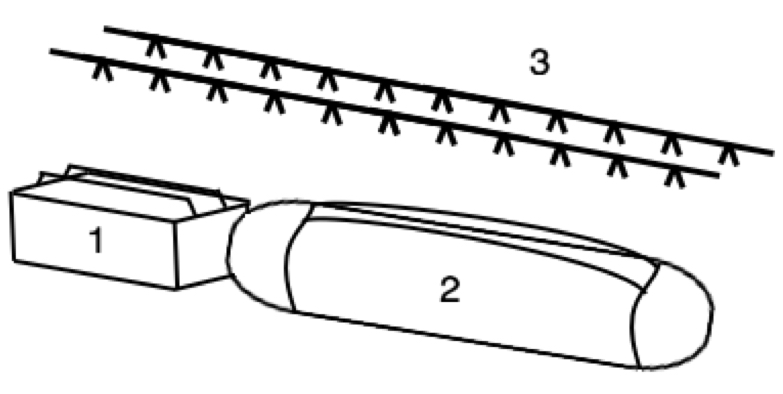
\includegraphics[width = .5\textwidth]{CommandDataHandling/Figures/Payload_module}
    \caption{Schematic example of payload mounting system}
    \label{fig:payl_moun_syst}
\end{figure}




\subsection{Payload Modules}
In this section, a short discussion on suggested payload modules for the different mission profiles will be given. The payload modules \textit{will not} be designed into full detail; however, components such as cameras are preferably chosen such that they are easily compatible with the Pixhawk flight control system. A modular clicking system will be installed, so that it is possible to drop (part of) the payload.

\begin{enumerate}
\item	\textbf{Search and rescue and support to disaster relief operations.} This requires a module that is able to locate the person(s) in need, and drop a help module. The difficulty in this module is that it will be dropped, so if an extra camera or battery is needed, they should be put in a separate module. As the object avoidance system that was chosen in \autoref{tab:avio_subs} is very powerful, that could also be used to locate the payload dropping location. The payload then only contains a care package or buoy. Velocity and range are most important here, but a mission specific trade-off should be made between those and payload capacity.
\item	\textbf{Precision agriculture by monitoring of cattle and crops.} For this type of mission, high-quality camera equipment is required. Endurance is the most important feature for this mission type, so an extra battery will also be installed. A camera that takes images at a high frequency should be selected, so it is possible to still generate lift using the wings.
\item \textbf{Transportation of parcels at sea and on land.} This type of mission requires large range. Therefore it will probably make use of a separate battery payload module and parcel module, where maximum battery size is dependent on payload size.
\item \textbf{Inspection of extensive industrial assets and infrastructures such as railways, high-tension powerlines, pipelines, wind farms, etc.} This type of mission requires similar equipment as mission 2. The difference is that this mission type documents long-range objects, while the agricultural one should cover large areas. Therefore, range is very important in this mission type. It will also make use of high-quality camera equipment and if possible and extra battery module.
\item 	\textbf{Transportation of organs for transplants.} In the case of transporting organs, high velocity is very important. The payload should be well-protected, which means it will probably be light, yet large. Some room might be available for extra batteries. The payload will not be dropped, but the UAV will land for unloading, so a cooling case could be designed for this means.
\end{enumerate}


\section{Communication Flow Diagram}
\label{sec:comm_flow_diag}

In this section, the communication flow diagram is illustrated in \autoref{fig:comm_flow_diag}. It illustrates the flow to and from the UAV system to the environment. 

\begin{figure}[h]
    \centering
    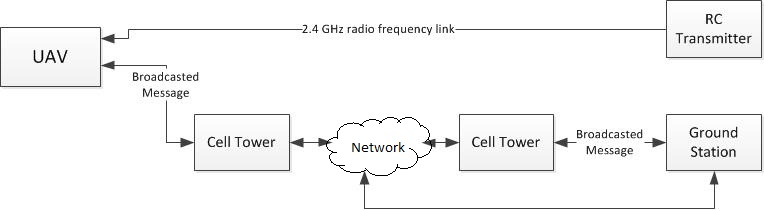
\includegraphics[width=\textwidth]{./CommandDataHandling/Figures/CommFlowDiagram.jpg}
    \caption{Communication Flow Block Diagram}
    \label{fig:comm_flow_diag}
\end{figure}

As explained in \autoref{sec:tele_syst}, the telemetry system consists of two different links, a direct link between the UAV and the control station using radio frequency and an indirect link using cellular technology. The radio frequency link is a one-way link to only send control commands to the flight controller. As seen in \autoref{fig:comm_flow_diag}, data send using the mobile network is first broadcasted through the air until it reaches a cell tower. Using the routing information on the IP packet, the data is either routed directly towards the ground station (in case it is connected to the internet) or to the closest cell tower from the ground station (in case it is connected via the mobile network). In the latter case, the cell tower broadcasts the message and the ground station can receive it. 

\section{Data Handling Block Diagram}
\label{sec:data_hand_bloc_diag}

In this section, the data handling block diagram is depicted in \autoref{fig:data_hand_bloc_diag}. The main purpose of this diagram is to illustrate the different data flows across the system. Furthermore it depicts the sample rates and processing speeds. 

\begin{figure}[h]
    \centering
    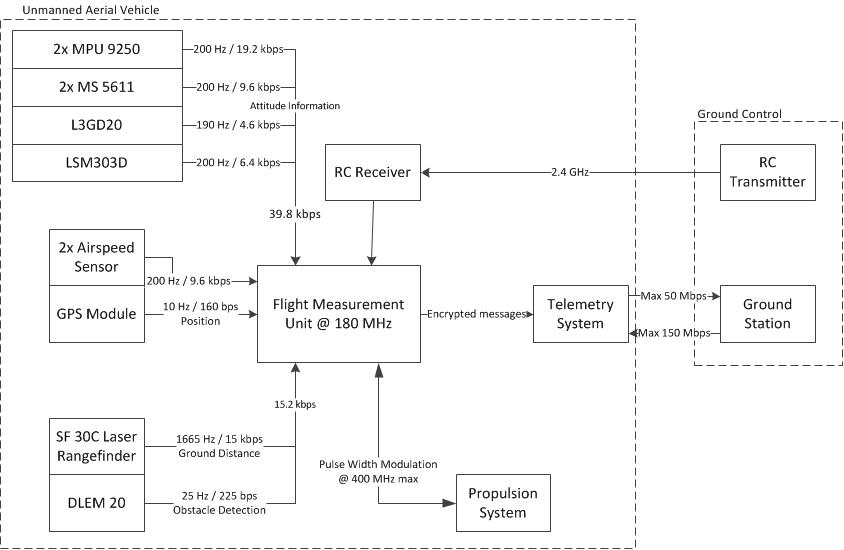
\includegraphics[width=0.8\textwidth]{./CommandDataHandling/Figures/DataDiagram.jpg}
    \caption{Data Handling Block Diagram}
    \label{fig:data_hand_bloc_diag}
\end{figure}

The attitude sensors can sample the information at different rates, however more sampling results in a bigger data flow and higher required processing power. It was assumed that sampling attitude information at a speed of 200 Hz results in a good overview of the UAV attitude. The sampling rates for the object avoidance, ground distance and GPS measurements are set to their maximum sampling rate. The frequency at which commands can be send to the propulsion system is limited by the physical link, in this case 400 MHz, which can however never be achieved due to the bottleneck set by the flight measurement unit of 180 MHz. The down- and uplink speeds of the telemetry system are their maxima and only achievable if the network is not congested. 

All sensors (position, attitude and object/ground avoidance) have a total data rate of 56 kbps. Some minor headers are added to the packages after processing due to the message authentication code and routing information, however the end data rate is orders of magnitude lower than the total achievable rate of 50 Mbps. This means enough margin is provided for the payload data rate and minor network congestion.   


\section{H/W \& S/W Block Diagrams}
\label{sec:hw_sw_bloc_diag}

In this section, the hardware and software diagrams are represented in Figures \ref{fig:hwdia} and \ref{fig:swdia}. As can be seen, they are are closely related. The hardware diagram focuses on the different physical interfaces used in the UAV and shows the different types of link between each interface. The software diagram illustrates the software that processes the data of each interface. 

\begin{figure}[h]
    \centering
    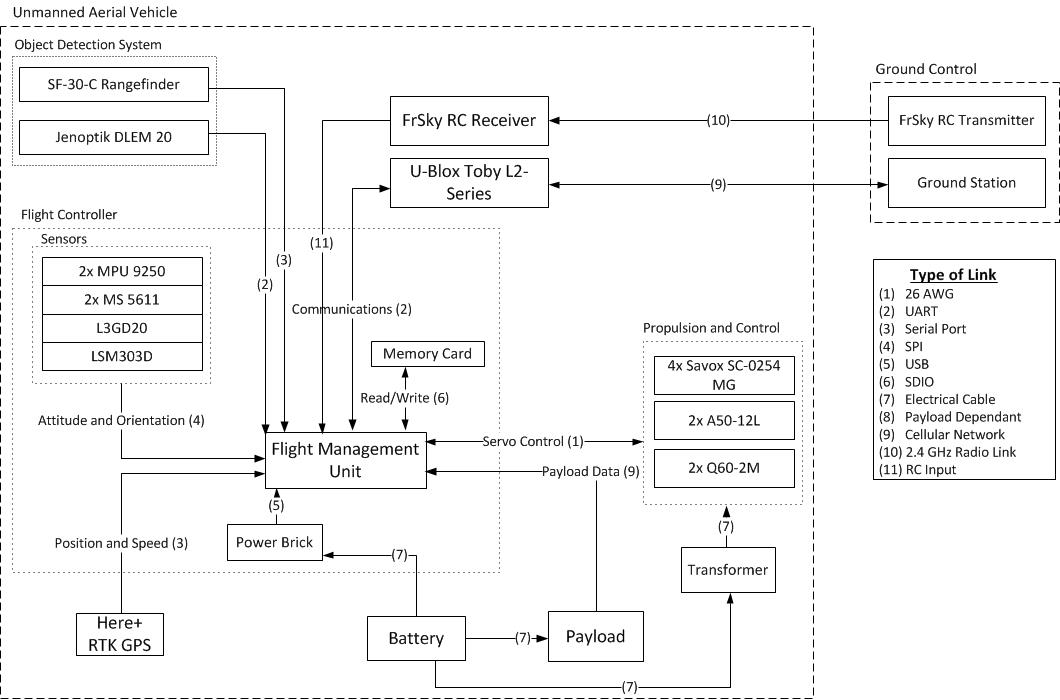
\includegraphics[width=.8\textwidth]{./CommandDataHandling/Figures/HWdiagram.jpg}
    \caption{Hardware Block Diagram}
    \label{fig:hwdia}
\end{figure}

\begin{figure}[h]
    \centering
    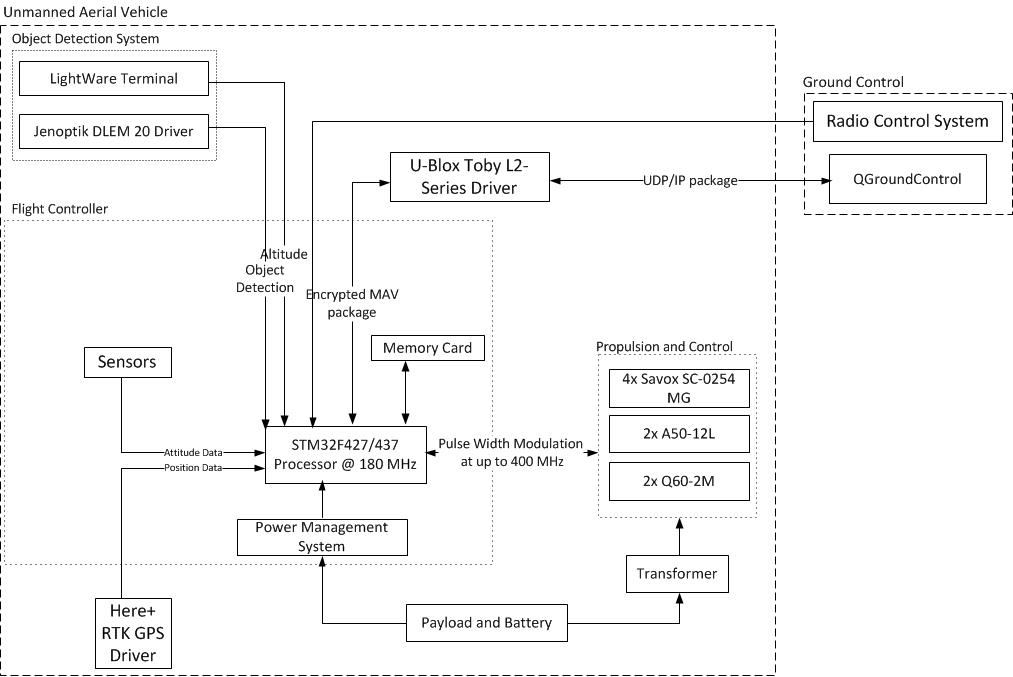
\includegraphics[width=.8\textwidth]{./CommandDataHandling/Figures/SWdiagram.jpg}
    \caption{Software Block Diagram}
    \label{fig:swdia}
\end{figure}

As seen in both diagrams, the central part of the system is the flight management unit. It is the processor used for autonomous flight control and to handle the data inside the system. With the exception of the propulsion and control system, all internal interfaces are connected to it and powered by it. Power related aspects are managed by the power brick. It regulates the voltage and current in order to prevent damage like burnout. It also monitors the power consumption and sends battery specific data to the flight management unit. 
The propulsion and control system in turn is powered by the battery itself. Each engine however has a separate transformer in order to reduce the battery voltage to its operational voltage. 